\chapter{System Design- The Box}

The Box is a stand alone, modular incubator that will be used to let certain SE3D experiments culture over an extended period of time. It will provide a custom lighting environment that allows consistent lighting conditions for the camera to effectively document the experiments. The box also will have temperature control capabilities to adjust temperature levels for each of the relevant SE3D experiments. The box will support nine petri dishes at one time.

\begin{figure}[H]
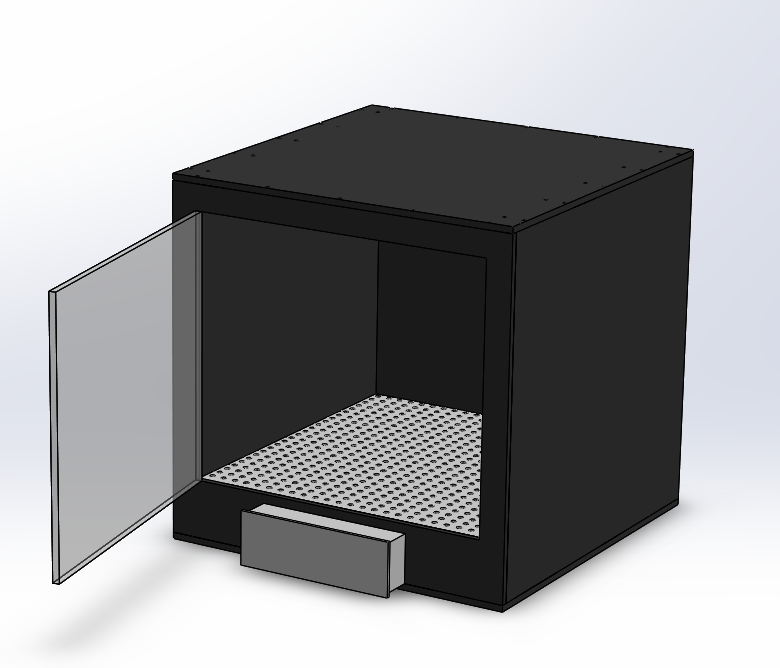
\includegraphics[scale=0.5]{box}
\caption{\label{figure:box} Initial Incubator Prototype}
\end{figure}

Figure \ref{figure:box} shows a initial drawing of the plans for the physical incubating box. At the top of the box, there will be a touch screen that allows users to interact with the controls of The Box.

% =======================================================================

% =======================================================================


% =======================================================================

% =======================================================================
\section{Conceptual Model}

The user interface for The Box consists of screens in which the user can configure the box’s settings for the current experiment, begin and end experiments, and download images that are collected during the experiment. The user interface shall perform the following: 

\begin{enumerate}
	\item	Run off of a microcomputer
	\item	Allow users to choose custom light, temperature, and image capture settings
	\item   Allow users to save a set of environment settings
	\item	Allow users to load a previously saved environment 
	\item	Organize all images from a single experiment into a folder per petri dish so that they each can be exported to USB 

\end{enumerate}

\begin{figure}[H]
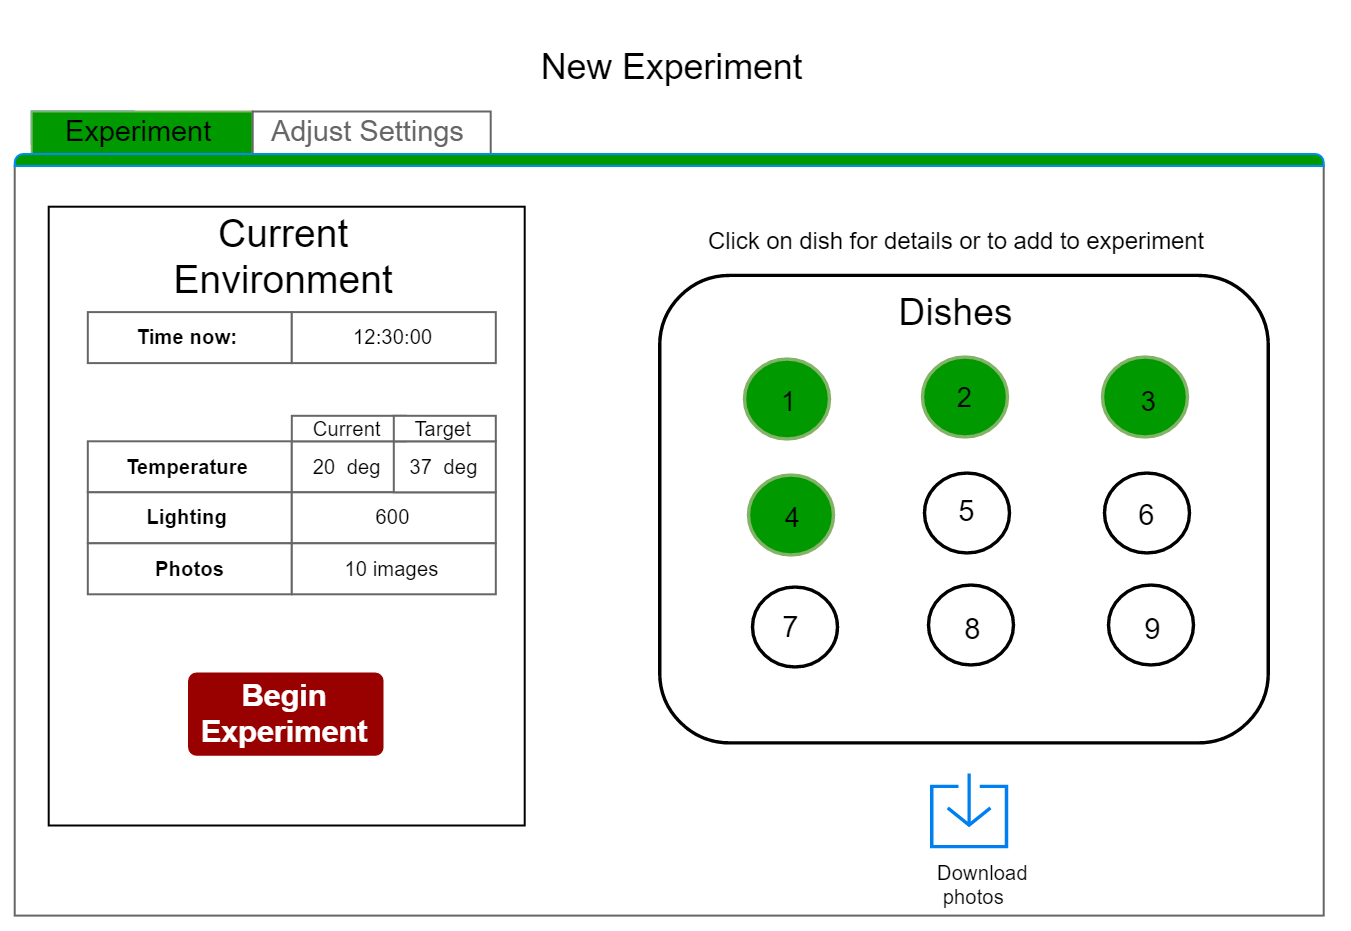
\includegraphics[scale=0.5]{ui-home-screen}
\caption{\label{figure:ui-home} Mock up of home screen}
\end{figure}

The user interface mock-ups shown in Figures \ref{figure:ui-home} through \ref{figure:ui-image} step through a typical sequence of steps a user would take when using the system. The first screen show, in Figure \ref{figure:ui-home}, is the default home screen that is shown when a experiment is not running. The home screen shows current environment status of the box. If a user would like to begin a new experiment, he would first select the dishes that will be initially placed into the incubator by clicking on each numbered circle that corresponds to a specific location inside of the physical box. Figure \ref{figure:ui-home} shows dishes 1-4 will be present in the experiment. 

\begin{figure}[H]
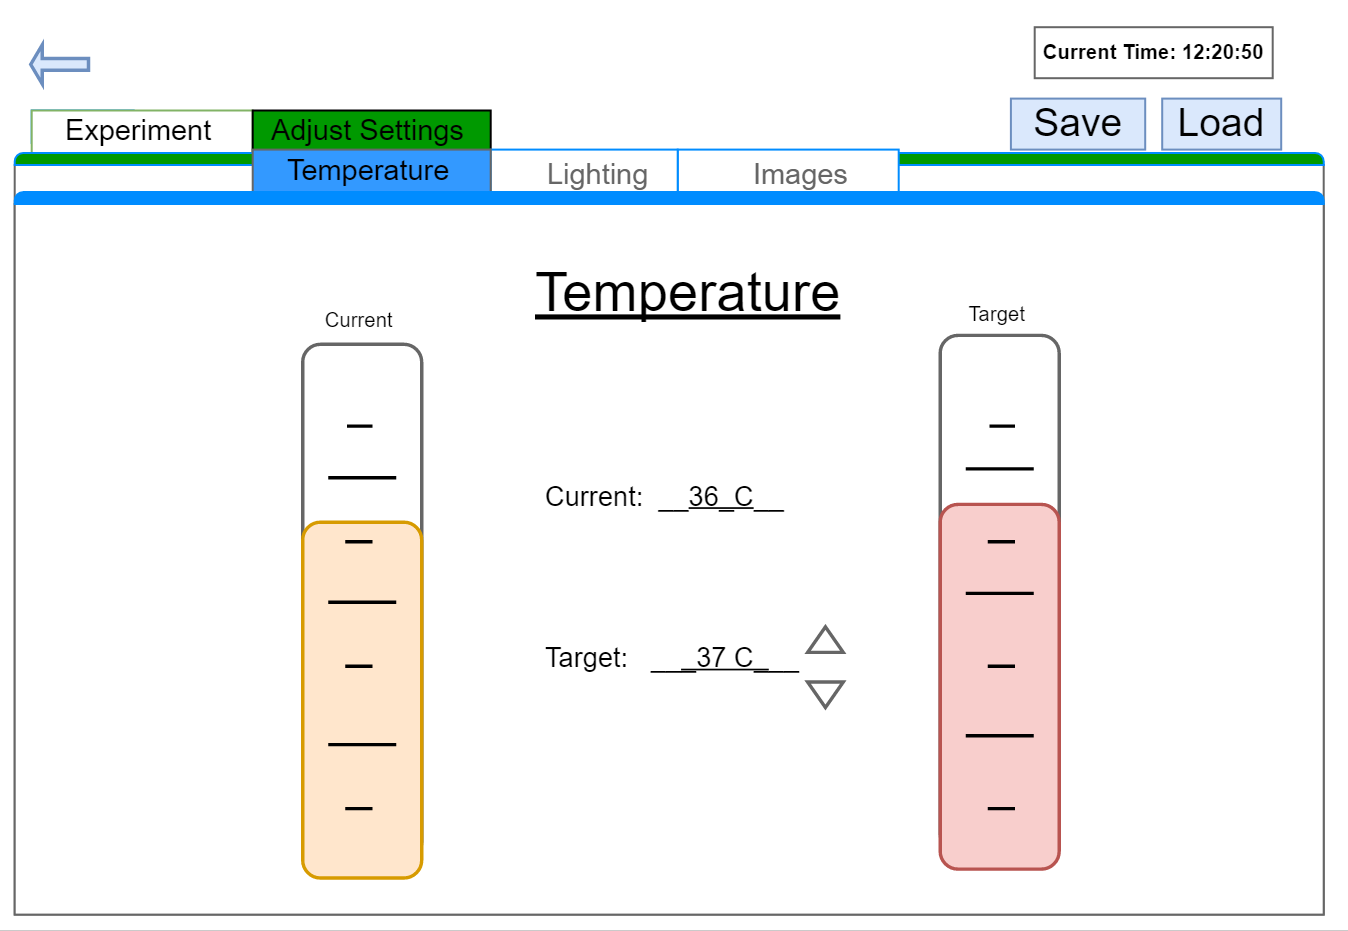
\includegraphics[scale=0.5]{ui-temp}
\caption{\label{figure:ui-temp} Mock up of temperature setting}

\end{figure}

\begin{figure}[H]
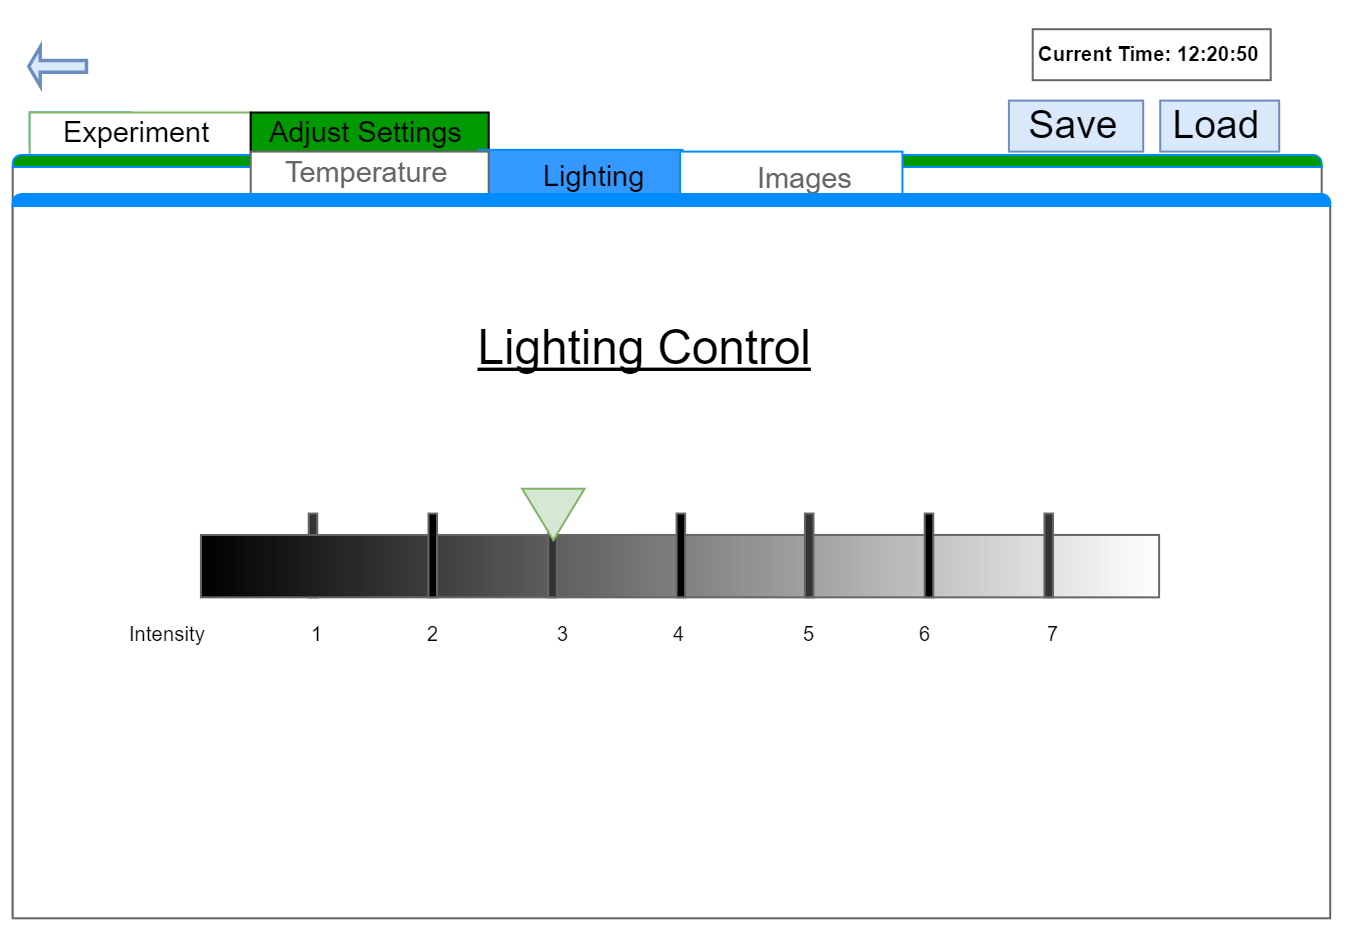
\includegraphics[scale=0.5]{ui-light}
\caption{\label{figure:ui-light} Mock up of light intensity setting}
\end{figure}

\begin{figure}[H]
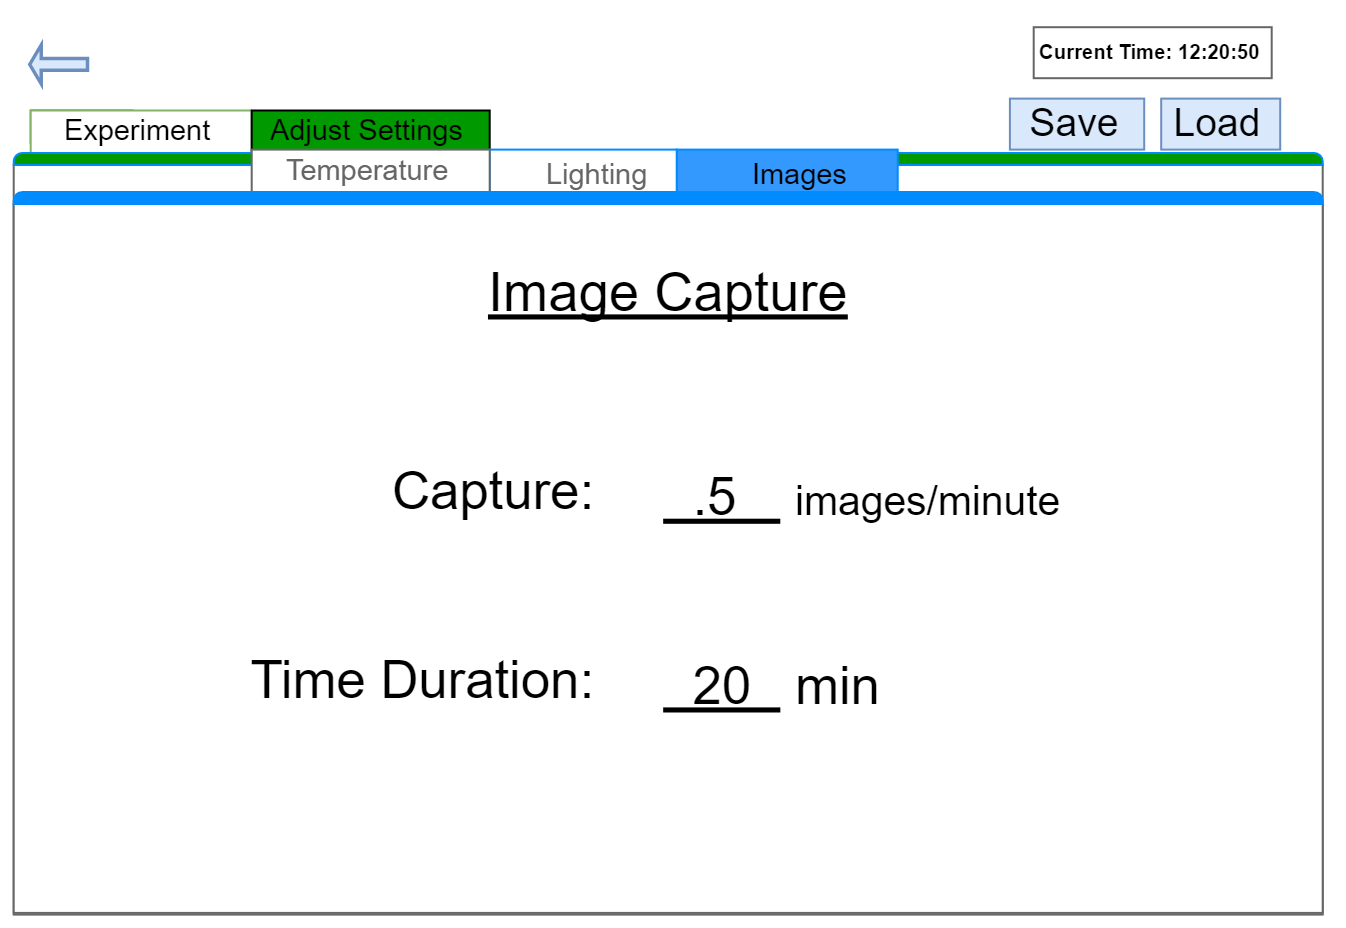
\includegraphics[scale=0.5]{ui-image}
\caption{\label{figure:ui-image} Mock up of image capture setting}
\end{figure}


Next, to customize the environment, the user would click adjust settings to be taken to the settings panel, shown in Figures \ref{figure:ui-temp} through \ref{figure:ui-image}. The user can choose to load a previously saved set of environment settings or provide a new set of environment settings. In each of these panels, the user can choose the appropriate temperature, light, and image capture settings for the system. After, he can choose to save the set of settings to be used in the future. 

\begin{figure}[H]
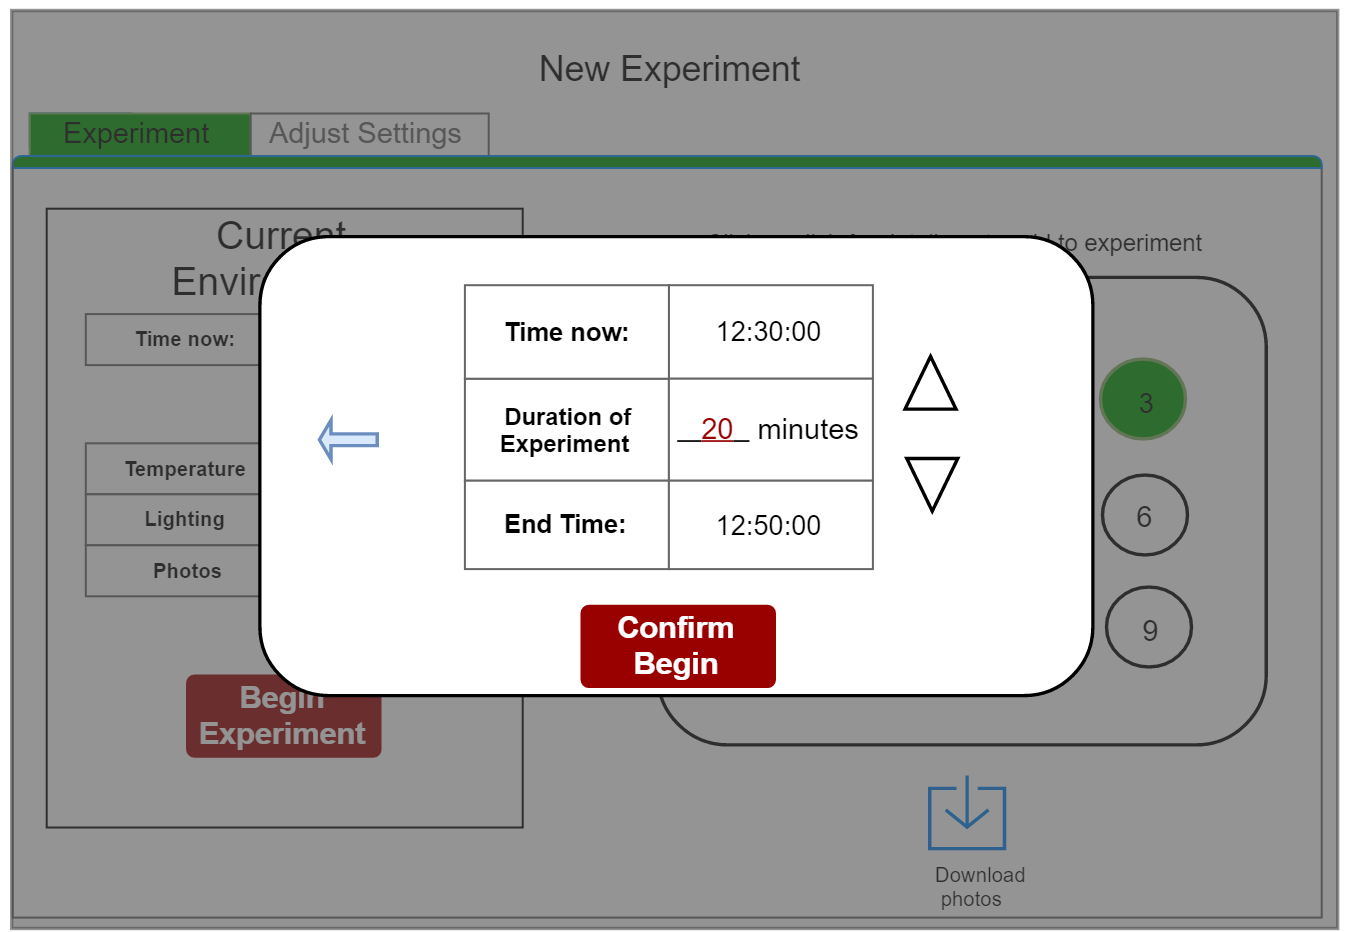
\includegraphics[scale=0.5]{ui-begin}
\caption{\label{figure:ui-begin} Mock up confirming experiment begin }
\end{figure}


Once the settings are appropriately chosen, the user navigates back to the home page to begin the experiment. The user clicks the `Begin Experiment' button and a confirmation screen will pop up to allow users to specify how long the incubating box will maintain the environment. This is shown in Figure \ref{figure:ui-begin}.


\begin{figure}[H]
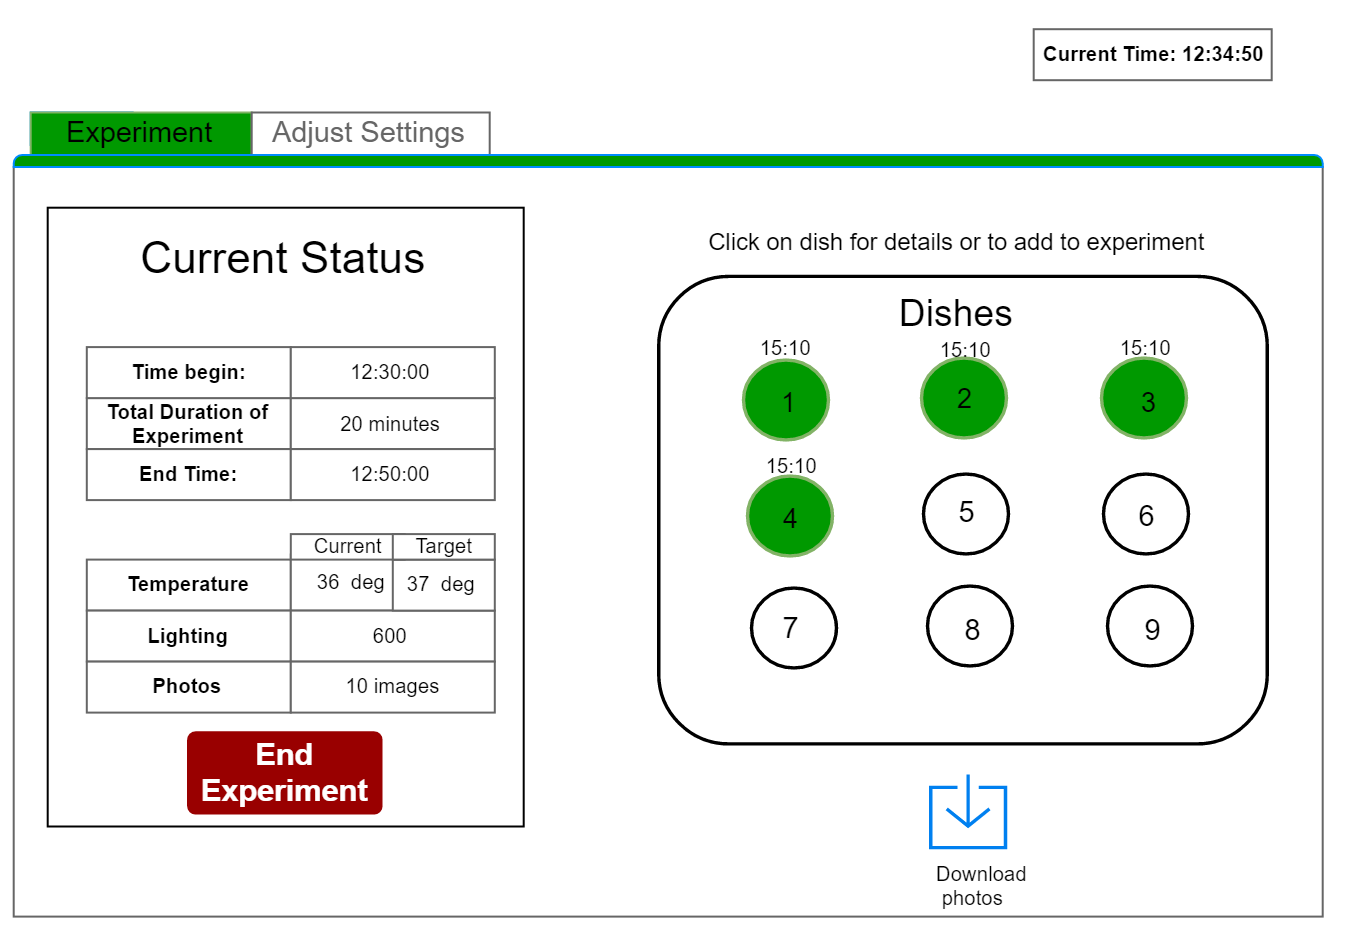
\includegraphics[scale=0.5]{ui-status-1}
\caption{\label{figure:ui-status} Mock up of status screen during an experiment}
\end{figure}

\begin{figure}[H]
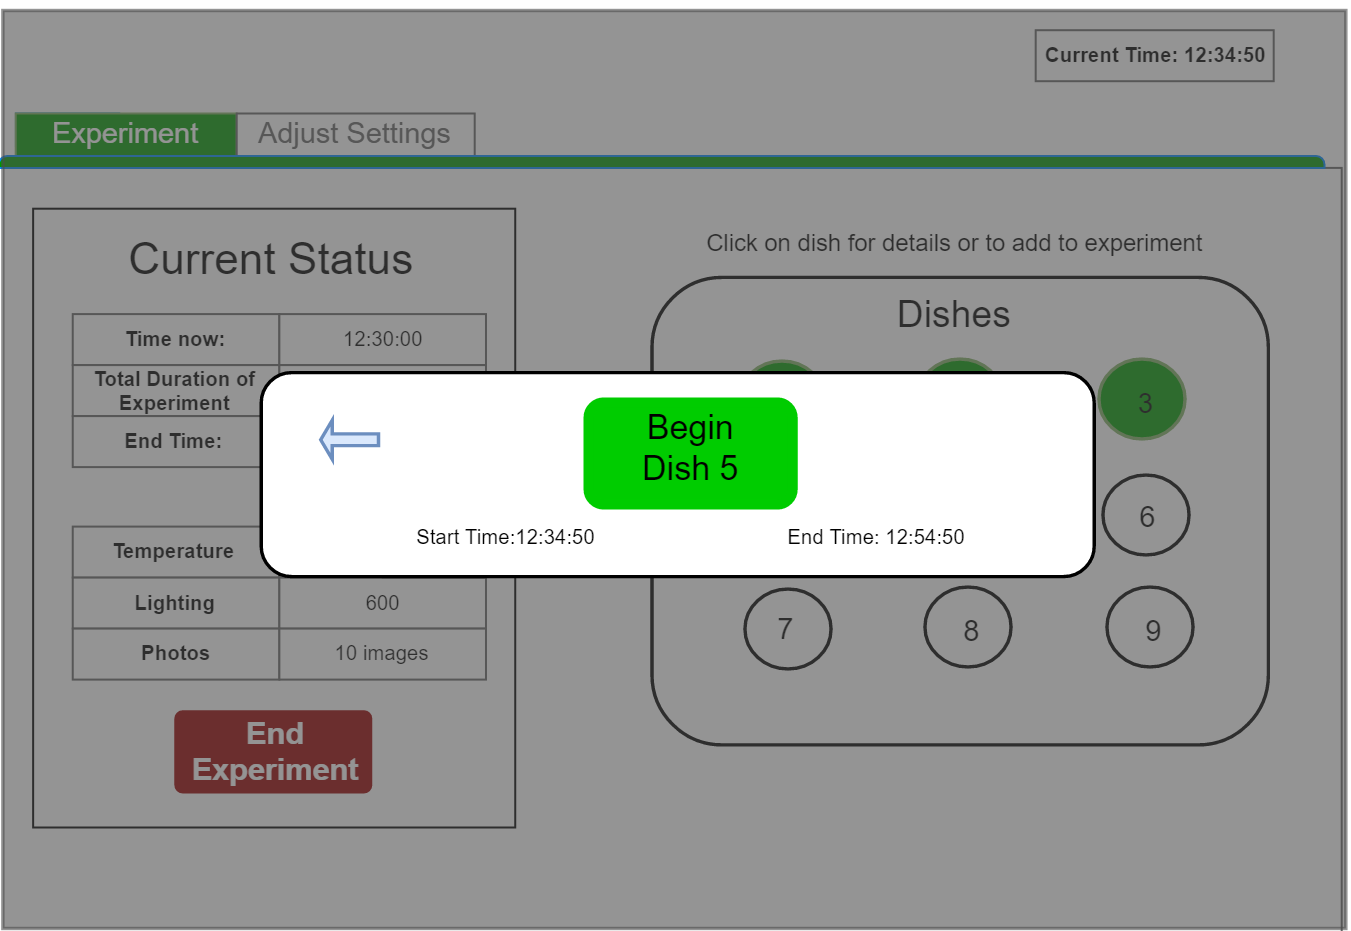
\includegraphics[scale=0.5]{ui-add-dish}
\caption{\label{figure:ui-add} Mock up of how a dish is added in the middle of an experiment}
\end{figure}

\begin{figure}[H]
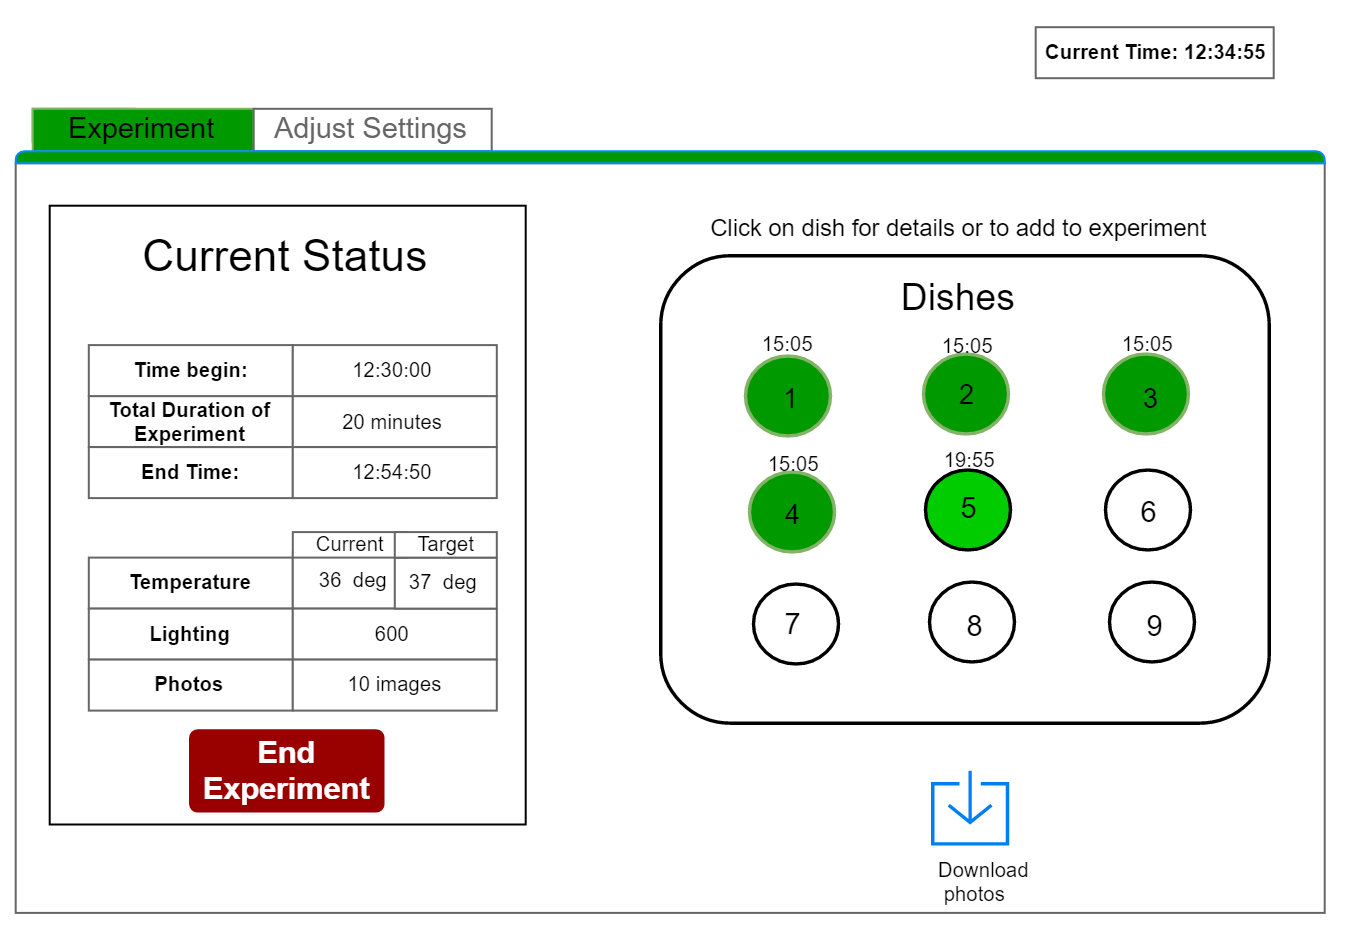
\includegraphics[scale=0.5]{ui-after-add}
\caption{\label{figure:ui-after-add} Mock up of how current status screen reflects addition of a dish}
\end{figure}

As seen in Figure \ref{figure:ui-status}, users will be able to monitor the experiment in real time and see how much time is left in the experiment as well as the current incubator conditions. If another dish needs to be added into the incubator in the middle of a running experiment, the user will add the dish into the box, then click on the corresponding circle on the screen. Figure \ref{figure:ui-add} shows Dish 5 being added into the experiment.  After the dish is added, the current staus screen is updated appropriately to reflect the change- specifically in the duration of experiment and end time sections as well as in the `Dishes' graphic. This is show in Figure \ref{figure:ui-after-add}.


\begin{figure}[H]
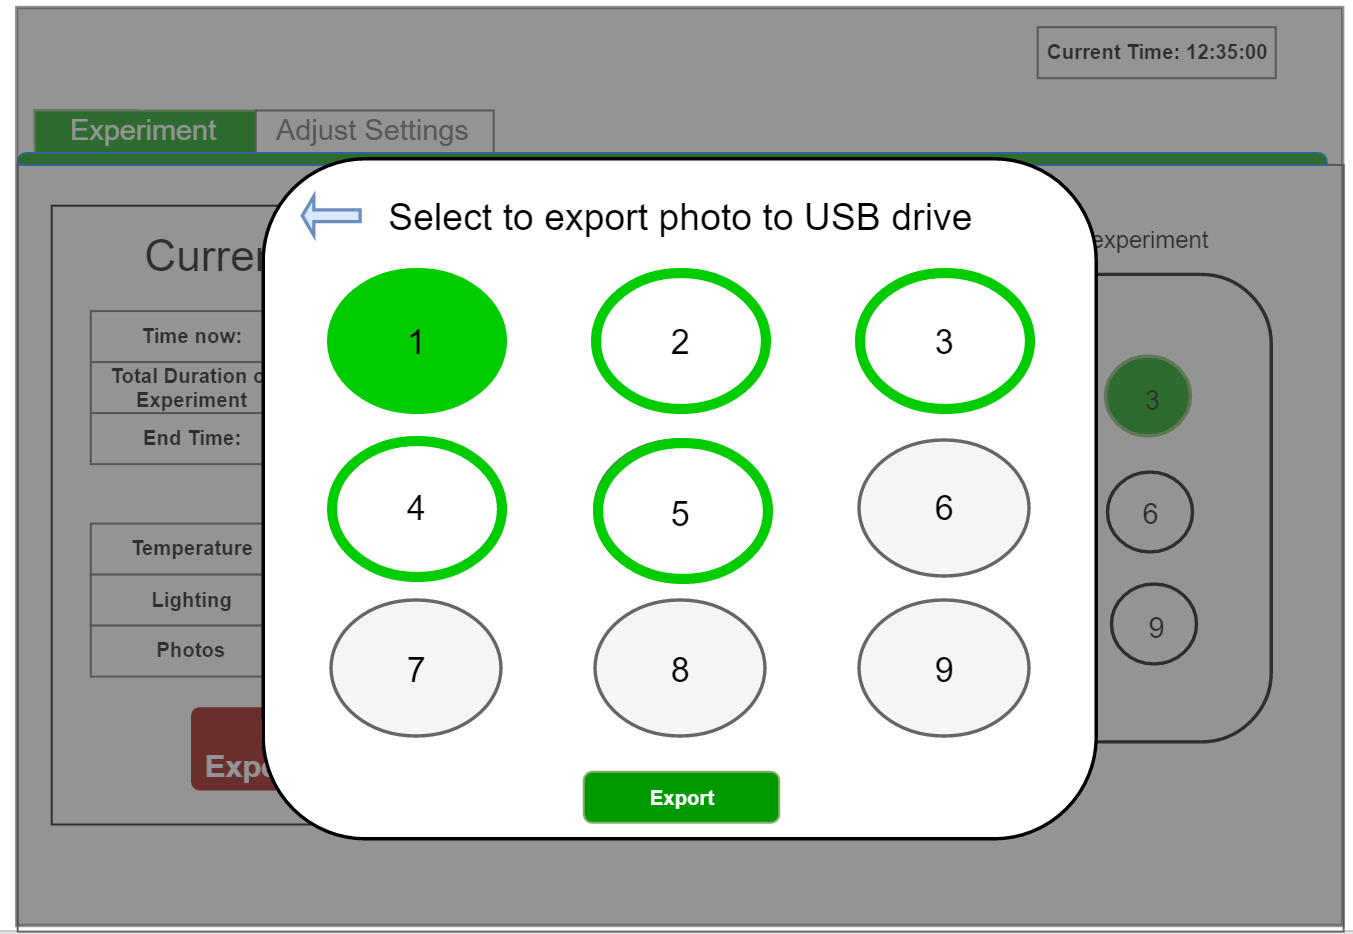
\includegraphics[scale=0.5]{ui-export}
\caption{\label{figure:ui-export} Mock up of export images to a USB drive}
\end{figure}

After an experiment is finished, users will export the images captured by USB. After a USB drive is inserted and recognized by the system, the user can click `Download Photos' on the status screen. A pop-up will allow the user to choose which dish's images the user would like to export. In Figure \ref{figure:ui-export}, the images of Dish 1 will be exported to the USB drive.



% =======================================================================

% =======================================================================
\section{Technologies Used}
	\begin{itemize}
	\item Git: A commonly used version control system. Git allows distributed work flow with high data integrity.
	\item Raspberry PI: A small, commonly used open-source computer with large community support. The Raspberry PI has General Purpose Input/Output (GPIO) pins for interfacing with other devices as well as built in WIFI, Bluetooth, GPU with HDMI output, and USB support.
	\item Java - A class based, object oriented computer programming language that is used for general purpose computing. Java is commonly found in projects around the world.
	\end{itemize}

% =======================================================================

% =======================================================================
\section{Design Rationale}
\subsection{Justification of User Experience}

We decided a touch screen interface was the most effective solution for the most enjoyable user experience for both high school students and instructors. A touch screen interface provides better image quality and intuitive interaction for users. Users are familiar with touch screens because of the popularity of touch screen smart phones and other screens.

The user interface is optimized for a touch screen experience. Since users will be using fingertips to navigate the interface, instead of a mouse cursor or stylus, all functions are tied to simple and prominent buttons. We kept the interface as simple as possible, only showing options and information that are necessary. Since we anticipate that we will have about a 5 in. screen, a simpler interface allows users to more easily navigate the system. In addition, since our users will be high school students, limiting the options they have on each screen reduces confusion on what to do next and lowers the chance of error due to unintentional clicks of other buttons.

There is minimal direct user input of values to reduce the need for on-screen keyboards that can be hard to navigate on a small screen. Instead, numbers are increased or decreased with up and down arrows, images, text, and color highlighting are used for signaling if certain dishes are selected or in use, and sliders are used in configuration. Reducing direct user input reduces  the likelihood of human error.

We chose not to include preloaded experiment settings that users can choose from after speaking with Maya from SE3D. Allowing users to input their own settings provides more flexibility for the user to customize experiments and create their own experiments. Since there are only a few criteria to set- light, temperature, image capture, and duration of experiment- it does not add too much overhead in set-up time. Users will have the option to save a certain combination of environment settings to use in the future. Thus, the `preloaded experiment' feature is emulated here- an instructor could set up a desired environment before class begins and save it to the system. Students can then load the environment that was set up by their instructor. 


\subsection{Justification of Technologies Used}
\begin{itemize}
	\item Git: Git was chosen because of its ability to store nearly any type of electronic materials such as images, source code, and documentation. It is commonly used in industry and is well supported. It allows the developers to work concurrently on various parts of the project which results in much faster completion times. Finally, because it is a version control system we can easily reference old code and track changes.

	\item Raspberry Pi: The Pi was chosen for the box because it incorporates sensor control and built in compatibility for cameras at an extremely low price point of \$35. It has a large community of developers that allow for support of external devices Because it is a full computer with a dedicated Graphical Processing Unit (GPU) it has integrated support for high resolution monitors with touch screens. It also has a filesystem for saving photos and onboard USB interfaces to exporting.

	\item Java - Java was used because it is natively supported on the Raspberry Pi and has built in library support for filesystem manipulation, camera use, and GPIO. In addition, Java has many integrated graphical libraries which is necessary for GUI design.
\end{itemize}
